\documentclass[dvipdfmx,11pt]{beamer}
%\graphicspath{{fig_tab/os_presentation/20201215/}}
\usepackage{lipsum}
\usetheme{Verona}
\usepackage{bxdpx-beamer}
\usepackage{pxjahyper}
\usepackage{minijs}
\usepackage{mathpazo}
\usepackage{amsmath,amssymb}
\usepackage{graphicx}
\usepackage{array}
\usepackage{tikz}
\usepackage{wrapfig}
\usepackage{float}
\usepackage{here}
\usepackage{lscape}
\usepackage{ascmac}
\usepackage{tabularx}
\renewcommand{\kanjifamilydefault}{\gtdefault}
\hypersetup{% hyperrefオプションリスト
 setpagesize=false,
 bookmarksnumbered=true,%
 bookmarksopen=true,%
 colorlinks=true,%
 linkcolor=blue,
 citecolor=blue,
 urlcolor = magenta
}
\setbeamertemplate{navigation symbols}{}

\title[Calderon, Fouka, and Tabellini (2022)]{Racial Diversity and Racial Policy Preferences: \\
The Great Migration and Civil Rights}
\subtitle{Calderon, Fouka, and Tabellini (2022)}
\author{Reviewed by Reio TANJI}
\date[6/12/2022 OS Seminar]{July 12th, 2022 \\ Ohtake-Sasaki Seminar}
\institute[]{Osaka University, Graduate School of Economics}

\begin{document}

\begin{frame}\frametitle{}
\titlepage
\end{frame}

\begin{frame}{Abstract}
  \begin{itemize}
    \item Research Question: Is the Great Migration is causally linked with support for civil rights?
    \begin{itemize}
      \item Between 1940 and 1970, more than 4 million African Americans moved from the South to the North of the US.
      \item At the same period witnessed the struggle and eventual success of the civil rights movements.
    \end{itemize}
    \item The (Second) Great Migration: Shift-share IV of Black inflows
    \begin{itemize}
      \item raised support for the Democratic Party
      \item increased Congress members' propensity to promote civil rights legislation
      \item encouraged pro-civil rights activism outside the US South
    \end{itemize} 
  \end{itemize}
\end{frame}

\frame{\tableofcontents}

\section{Introduction}
\frame{\sectionpage}

\begin{frame}{}
  
\end{frame}

\begin{frame}{}
  \begin{figure}
    \centering
    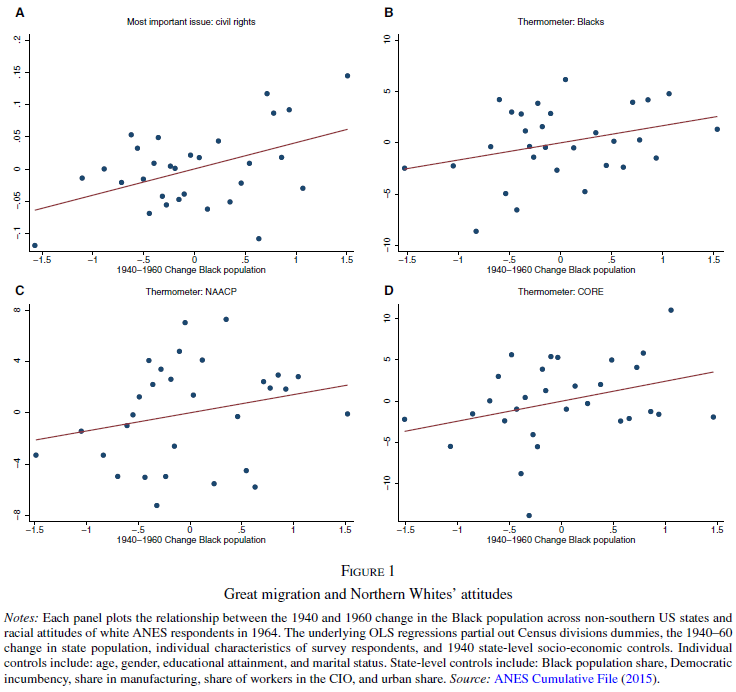
\includegraphics[scale = .45]{fig_tab/os20220708/F1.png}
  \end{figure}
\end{frame}

\section{Historical Background}
\frame{\sectionpage}

\section{Data}
\frame{\sectionpage}

\section{Empirical Strategy}
\frame{\sectionpage}

\section{Main Results}
\frame{\sectionpage}

\section{Mechanisms}
\frame{\sectionpage}

\section{Conclusions}
\frame{\sectionpage}

\end{document}
